\chapter{Biosynthesen en de geïntegreerde cel}\label{ch:b1:biosyntheses-integration}

Om acht uur 's ochtends zet een lever de suiker van het ontbijt om in \omterm{def:b1:carbohydrates:polysaccharide}{glycogeen} en
\omterm{def:b1:lipids:triglyceride}{vet}; om drie uur de volgende nacht maakt diezelfde lever suiker uit de \omterm{def:b1:proteins:aminoacid}{aminozuren}
van spier en giet die in het bloed voor een brein dat negen uur niets heeft
gegeten. Aan de \omterm{def:b1:enzymes:enzyme}{enzymen} is niets veranderd; wat er is veranderd, is welke ervan
aanstaan. De vorige hoofdstukken haalden de moleculen van de \omterm{def:b1:cell-unit-of-life:cell}{cel} uit elkaar; dit
hoofdstuk zet ze in elkaar --- de synthese van suikers, \omterm{def:b1:carbohydrates:polysaccharide}{glycogeen}, \omterm{def:b1:lipids:triglyceride}{vetten} en
\omterm{def:b1:proteins:aminoacid}{aminozuren} --- en vraagt daarna hoe een \omterm{def:b1:cell-unit-of-life:cell}{cel}, en een \omterm{def:b1:organism-environment:organism}{organisme}, op elk moment
beslissen welke routes lopen. Het antwoord is een kleine reeks gedeelde
munteenheden, enkele \omterm{def:b1:enzymes:enzyme}{enzymen} op de kruispunten, en hormonen die elke \omterm{def:b1:cell-unit-of-life:cell}{cel} de
toestand van het geheel vertellen.

\section{Wat een synthese nodig heeft}

\begin{proposition}[De drie eisen van het anabolisme]\label{prop:b1:biosyntheses-integration:needs}
\index{anabolisme}
Elke biosynthese heeft \emph{koolstofskeletten} nodig, ontleend aan een handvol
tussenproducten van de \omterm{def:b1:respiration-fermentation:glycolysis}{glycolyse} en de \omterm{def:b1:respiration-fermentation:krebs}{krebscyclus}; \emph{reducerende kracht},
geleverd als \omterm{def:b1:biosyntheses-integration:ppp}{NADPH}; en \emph{energie}, geleverd als \omterm{def:b1:water-small-molecules:atp}{ATP}. Het katabolisme en het
anabolisme komen daarom op dezelfde kruispunten samen --- glucose-6-fosfaat,
triosefosfaat, pyruvaat, \omterm{def:b1:respiration-fermentation:pdh}{acetyl-CoA}, $\alpha$-ketoglutaraat, oxaalacetaat --- maar
lopen bij de onomkeerbare stappen over afzonderlijke \omterm{def:b1:enzymes:enzyme}{enzymen}, zodat elke richting
apart kan worden geschakeld, en zij gebruiken voor hun elektronen afzonderlijke
\omterm{def:b1:enzymes:enzyme}{co-enzymen}: NADH, geoxideerd gehouden, om in het katabolisme elektronen weg te
nemen; \omterm{def:b1:biosyntheses-integration:ppp}{NADPH}, gereduceerd gehouden, om ze bij de synthese af te geven.
\end{proposition}

\begin{definition}[De pentosefosfaatroute]\label{def:b1:biosyntheses-integration:ppp}
\index{pentosefosfaatroute}\index{NADPH}
De \emph{pentosefosfaatroute} van het \omterm{def:b1:eukaryotic-cell:organelle}{cytosol} oxideert glucose-6-fosfaat tot
ribulose-5-fosfaat en $\mathrm{CO_2}$, waarbij twee $\mathrm{NADP^+}$ tot NADPH
worden gereduceerd; haar niet-oxidatieve tak zet vervolgens suikerfosfaten met
vijf, vier, zes en zeven koolstoffen in elkaar om, zodat de \omterm{def:b1:cell-unit-of-life:cell}{cel}
ribose-5-fosfaat voor \omterm{def:b1:nucleic-acids:nucleotide}{nucleotiden} kan maken wanneer zij pentosen nodig heeft,
NADPH wanneer zij reducerende kracht nodig heeft (vetsynthese, verdediging tegen
oxidanten), of beide, en de rest aan de \omterm{def:b1:respiration-fermentation:glycolysis}{glycolyse} kan teruggeven. Zij is de
belangrijkste bron van NADPH in dierlijke \omterm{def:b1:cell-unit-of-life:cell}{cellen}; bij planten leveren de
\omterm{prop:b1:photosynthesis:lightreactions}{lichtreacties} van de chloroplast overdag NADPH.
\end{definition}

\begin{omfigure}
\begin{tikzpicture}[font=\footnotesize, >=Stealth, line cap=round,
  hub/.style={draw, thick, rounded corners=3pt, fill=omDef!12, inner sep=3pt, align=center},
  prod/.style={draw, thick, rounded corners=3pt, fill=omExo!15, inner sep=3pt, align=center},
  fuel/.style={draw, thick, rounded corners=3pt, fill=omProp!15, inner sep=3pt, align=center}]
  \node[hub] (g6p) at (0,4.5) {glucose-6-P};
  \node[hub] (tp) at (0,2.8) {triose-P};
  \node[hub] (pyr) at (0,1.1) {pyruvaat};
  \node[hub] (accoa) at (0,-0.6) {acetyl-CoA};
  \node[hub] (krebs) at (0,-2.4) {krebscyclus\\ ($\alpha$-KG, OAA)};
  \draw[<->, thick] (g6p) -- (tp); \draw[<->, thick] (tp) -- (pyr); \draw[->, thick] (pyr) -- (accoa); \draw[->, thick] (accoa) -- (krebs);
  % left: stores and fuels in
  \node[fuel] (gly) at (-4.2,4.5) {glycogeen, zetmeel}; \draw[<->, thick] (gly) -- (g6p);
  \node[fuel] (lac) at (-4.2,1.1) {lactaat}; \draw[<->, thick] (lac) -- (pyr);
  \node[fuel] (fa) at (-4.2,-0.6) {vetzuren}; \draw[<->, thick] (fa) -- (accoa) node[pos=0.62, below=2pt, font=\scriptsize] {$\beta$-oxidatie / synthese};
  \node[fuel] (aa) at (-4.2,-2.4) {aminozuren}; \draw[<->, thick] (aa) -- (krebs) node[pos=0.4, below=2pt, font=\scriptsize] {transaminering};
  % right: products
  \node[prod] (ppp) at (4.3,4.5) {pentosefosfaatroute:\\ NADPH, ribose-5-P $\to$ nucleotiden}; \draw[->, thick] (g6p) -- (ppp);
  \node[prod] (glyc) at (4.3,2.8) {glycerol $\to$ lipiden}; \draw[->, thick] (tp) -- (glyc);
  \node[prod] (ala) at (4.3,1.1) {alanine, serine, glycine}; \draw[<->, thick] (pyr) -- (ala);
  \node[prod] (chol) at (4.3,-0.6) {cholesterol, steroïden;\\ ketonlichamen}; \draw[->, thick] (accoa) -- (chol);
  \node[prod] (glu) at (4.3,-2.4) {glutamaat, aspartaat\\ en hun families; heem}; \draw[<->, thick] (krebs) -- (glu);
  \draw[->, very thick, omThm] (1.4,-2.0) -- (1.4,0.65) node[pos=0.5, rotate=90, anchor=south, font=\scriptsize, omThm] {gluconeogenese};
\end{tikzpicture}

{\small De kruispunten van de stofwisseling. Zes knooppunten van de centrale routes
(blauw) ontvangen brandstoffen en voorraden (oranje) en leveren aan elke
biosynthese (groen). De \omterm{def:b1:biosyntheses-integration:gluconeogenesis}{gluconeogenese} (rood) loopt het midden van de kaart omhoog.}
\end{omfigure}

\section{Glucose maken: gluconeogenese}

\begin{definition}[Gluconeogenese]\label{def:b1:biosyntheses-integration:gluconeogenesis}
\index{gluconeogenese}
De \emph{gluconeogenese} maakt glucose uit voorlopers die geen \omterm{def:b1:carbohydrates:monosaccharide}{koolhydraat} zijn ---
lactaat, pyruvaat, glycerol en de koolstofskeletten van de meeste \omterm{def:b1:proteins:aminoacid}{aminozuren} ---
in de lever (en een beetje in de nier). Zij laat de \omterm{def:b1:respiration-fermentation:glycolysis}{glycolyse} achterwaarts lopen
langs haar zeven omkeerbare stappen en omzeilt de drie onomkeerbare met andere
\omterm{def:b1:enzymes:enzyme}{enzymen}: pyruvaat wordt gecarboxyleerd tot oxaalacetaat (in het \omterm{def:b1:eukaryotic-cell:mitochondrion}{mitochondrion}, één
\omterm{def:b1:water-small-molecules:atp}{ATP}) en gedecarboxyleerd tot fosfo-enolpyruvaat (één GTP);
fructose-1,6-bisfosfaat wordt gehydrolyseerd tot fructose-6-fosfaat;
glucose-6-fosfaat wordt gehydrolyseerd tot vrije glucose, die de \omterm{def:b1:cell-unit-of-life:cell}{cel} verlaat. Per
glucose: 6 ATP-equivalenten en 2 NADH, tegen de 2 \omterm{def:b1:water-small-molecules:atp}{ATP} die de \omterm{def:b1:respiration-fermentation:glycolysis}{glycolyse} oplevert ---
de prijs van een bergafwaartse weg bergop lopen.
\end{definition}

\begin{omfigure}
\begin{tikzpicture}[font=\footnotesize, >=Stealth, line cap=round,
  m/.style={draw, thick, rounded corners=3pt, inner sep=3pt, fill=omDef!10, align=center}]
  \node[m] (glc) at (0,5.2) {glucose};
  \node[m] (g6p) at (0,3.9) {glucose-6-P};
  \node[m] (f6p) at (0,2.6) {fructose-6-P};
  \node[m] (fbp) at (0,1.3) {fructose-1,6-bisP};
  \node[m] (pep) at (0,-0.5) {fosfo-enolpyruvaat};
  \node[m] (pyr) at (0,-1.9) {pyruvaat};
  \node[m] (oaa) at (5.2,-1.9) {oxaalacetaat};
  % glycolysis (down, left side)
  \draw[->, thick, omDef!70!black] (glc.west) ++(-0.2,0) -- ++(-1.0,0) |- (g6p.west) node[pos=0.25, left, font=\scriptsize, align=right] {hexokinase\\ ATP};
  \draw[->, thick, omDef!70!black] (f6p.west) ++(-0.2,0) -- ++(-1.0,0) |- (fbp.west) node[pos=0.25, left, font=\scriptsize, align=right] {PFK\\ ATP};
  \draw[->, thick, omDef!70!black] (pep.west) ++(-0.2,0) -- ++(-1.0,0) |- (pyr.west) node[pos=0.25, left, font=\scriptsize, align=right] {pyruvaatkinase\\ ATP gemaakt};
  \draw[<->, thick] (g6p) -- (f6p); \draw[<->, thick] (fbp) -- (pep) node[midway, right, font=\scriptsize] {omkeerbare stappen (gedeeld)};
  % gluconeogenesis (up, right side)
  \draw[->, thick, omThm] (g6p.east) ++(0.2,0) -- ++(1.0,0) |- (glc.east) node[pos=0.25, right, font=\scriptsize, align=left] {glucose-6-fosfatase\\ (alleen lever)};
  \draw[->, thick, omThm] (fbp.east) ++(0.2,0) -- ++(1.0,0) |- (f6p.east) node[pos=0.25, right, font=\scriptsize, align=left] {fructose-1,6-\\ bisfosfatase};
  \draw[->, thick, omThm] (pyr) -- (oaa) node[midway, below=3pt, font=\scriptsize] {pyruvaatcarboxylase, ATP};
  \draw[->, thick, omThm] (oaa) |- (pep.east);
  \node[anchor=south, font=\scriptsize, omThm] at (3.6,-0.4) {PEP-carboxykinase, GTP};
  \node[anchor=north, align=center, gray] at (1.0,-2.7) {blauw: glycolyse (omlaag); rood: de drie omleidingen van de gluconeogenese (omhoog)\\ kosten van één glucose uit twee pyruvaat: 4 ATP $+$ 2 GTP $+$ 2 NADH};
\end{tikzpicture}

{\small De \omterm{def:b1:respiration-fermentation:glycolysis}{glycolyse} en de \omterm{def:b1:biosyntheses-integration:gluconeogenesis}{gluconeogenese} delen zeven omkeerbare reacties en
verschillen bij drie onomkeerbare, die elk door een apart \omterm{def:b1:enzymes:enzyme}{enzym} worden omzeild.
Aparte \omterm{def:b1:enzymes:enzyme}{enzymen} betekenen aparte regeling: de lever kan de ene richting aanzetten en
de andere uitzetten.}
\end{omfigure}

\begin{proposition}[Wat wel en wat niet glucose kan worden]\label{prop:b1:biosyntheses-integration:cannot}
Lactaat, glycerol en de \omterm{def:b1:proteins:aminoacid}{aminozuren} die pyruvaat of tussenproducten van de
\omterm{def:b1:respiration-fermentation:krebs}{krebscyclus} opleveren (alle behalve leucine en lysine) kunnen in glucose worden
omgezet. \omterm{def:b1:lipids:fattyacid}{Vetzuren} kunnen dat bij dieren niet: hun $\beta$-oxidatie geeft
\omterm{def:b1:respiration-fermentation:pdh}{acetyl-CoA}, waarvan de twee koolstoffen de cyclus binnenkomen en als twee
$\mathrm{CO_2}$ vertrekken voordat er oxaalacetaat wordt gewonnen, zodat er geen
netto weg van \omterm{def:b1:respiration-fermentation:pdh}{acetyl-CoA} naar suiker bestaat. Planten, schimmels en bacteriën
bezitten de \emph{glyoxylaatcyclus}, een kortere weg die de twee decarboxyleringen
overslaat en een kiemend oliehoudend zaad zijn \omterm{def:b1:lipids:triglyceride}{vet} in de suiker laat omzetten die
zijn kiemplant nodig heeft. Een hongerend zoogdier moet zijn glucose daarentegen
uit \omterm{def:b1:proteins:peptide}{eiwit} maken.
\end{proposition}

\begin{example}[De coricyclus]\label{ex:b1:biosyntheses-integration:cori}
Een sprintende spier vergist \omterm{def:b1:carbohydrates:polysaccharide}{glycogeen} tot lactaat, dat het bloed in gaat; de lever
neemt het lactaat op, oxideert het tot pyruvaat, maakt er glucose van tegen 6 \omterm{def:b1:water-small-molecules:atp}{ATP}
per glucose, en geeft de glucose aan het bloed terug zodat de spier haar opnieuw
kan gebruiken. De spier heeft zonder zuurstof 2 \omterm{def:b1:water-small-molecules:atp}{ATP} per glucose gewonnen en een
rekening van 6 aan de lever doorgeschoven, die haar op haar gemak met zuurstof
betaalt: de ``zuurstofschuld'' van een sprint wordt grotendeels in de lever
afbetaald.
\end{example}

\section{Opslaan: glycogeen en vet}

\begin{definition}[Glycogeensynthese]\label{def:b1:biosyntheses-integration:glycogensynthesis}
Glucose wordt als \omterm{def:b1:carbohydrates:polysaccharide}{glycogeen} opgeslagen door glucose-6-fosfaat te activeren tot
\emph{UDP-glucose} (één UTP), dat het \emph{glycogeensynthase} aan de
niet-reducerende uiteinden van de bestaande boom toevoegt; een
\emph{vertakkingsenzym} knipt korte ketens los en hecht ze opnieuw aan om de
$\alpha(1{\to}6)$-vertakkingen te maken (\cref{ch:b1:carbohydrates}). Het synthase
en het fosforylase worden door dezelfde signalen in tegengestelde richting
geregeld: de fosforylering die het fosforylase aanzet, zet het synthase uit, zodat
de boom nooit tegelijk wordt gebouwd en afgebroken.
\end{definition}

\begin{definition}[Vetzuursynthese]\label{def:b1:biosyntheses-integration:fasynthesis}
\index{vetzuursynthese}
\omterm{def:b1:lipids:fattyacid}{Vetzuren} worden in het \omterm{def:b1:eukaryotic-cell:organelle}{cytosol} gemaakt uit \omterm{def:b1:respiration-fermentation:pdh}{acetyl-CoA} dat uit het \omterm{def:b1:eukaryotic-cell:mitochondrion}{mitochondrion} is
uitgevoerd. Het \emph{acetyl-CoA-carboxylase}, de geregelde stap, carboxyleert het
(één \omterm{def:b1:water-small-molecules:atp}{ATP}) tot malonyl-CoA; het \emph{vetzuursynthase} voegt daarna telkens twee
koolstoffen uit malonyl-CoA aan een groeiende keten toe en reduceert elke
toevoeging met twee \omterm{def:b1:biosyntheses-integration:ppp}{NADPH}, tot palmitaat (C16) wordt vrijgegeven: 8 \omterm{def:b1:respiration-fermentation:pdh}{acetyl-CoA}, 7
\omterm{def:b1:water-small-molecules:atp}{ATP} en 14 \omterm{def:b1:biosyntheses-integration:ppp}{NADPH} per palmitaat. Verlenging en ontverzadiging in het \omterm{def:b1:eukaryotic-cell:endomembrane}{endoplasmatisch
reticulum} maken de overige zuren; verestering met glycerol-3-fosfaat (uit
triosefosfaat) maakt \omterm{def:b1:lipids:triglyceride}{triglyceriden}. De route is niet de omgekeerde
$\beta$-oxidatie: andere \omterm{def:b1:enzymes:enzyme}{enzymen}, een ander compartiment, malonyl-CoA in plaats van
\omterm{def:b1:respiration-fermentation:pdh}{acetyl-CoA}, \omterm{def:b1:biosyntheses-integration:ppp}{NADPH} in plaats van $\mathrm{FADH_2}$ en NADH --- en malonyl-CoA
blokkeert het transport van \omterm{def:b1:lipids:fattyacid}{vetzuren} het \omterm{def:b1:eukaryotic-cell:mitochondrion}{mitochondrion} in, zodat een \omterm{def:b1:cell-unit-of-life:cell}{cel} niet
tegelijk \omterm{def:b1:lipids:triglyceride}{vet} maakt en verbrandt.
\end{definition}

\begin{example}[Vet uit suiker]\label{ex:b1:biosyntheses-integration:fatfromsugar}
Een lever die meer glucose krijgt dan zij als \omterm{def:b1:carbohydrates:polysaccharide}{glycogeen} kan opslaan maakt \omterm{def:b1:lipids:triglyceride}{vet}:
glucose naar pyruvaat naar \omterm{def:b1:respiration-fermentation:pdh}{acetyl-CoA} (waarbij een derde van de koolstof als
$\mathrm{CO_2}$ verloren gaat en er \omterm{def:b1:water-small-molecules:atp}{ATP} wordt gewonnen), \omterm{def:b1:respiration-fermentation:pdh}{acetyl-CoA} naar palmitaat
ten koste van dat \omterm{def:b1:water-small-molecules:atp}{ATP} en van \omterm{def:b1:biosyntheses-integration:ppp}{NADPH} uit de \omterm{def:b1:biosyntheses-integration:ppp}{pentosefosfaatroute}, palmitaat naar
\omterm{def:b1:lipids:triglyceride}{triglyceride} dat naar het vetweefsel wordt verscheept. Zo'n \qty{15}{\%} van de
energie van de suiker gaat bij de omzetting verloren; de rest wordt negen keer
compacter opgeslagen dan \omterm{def:b1:carbohydrates:polysaccharide}{glycogeen} (\cref{ch:b1:lipids}). Het omgekeerde --- \omterm{def:b1:lipids:triglyceride}{vet}
naar suiker --- is onmogelijk.
\end{example}

\section{Stikstof: aminozuren en nucleotiden}

\begin{definition}[Stikstofassimilatie, transaminering]\label{def:b1:biosyntheses-integration:nitrogen}
\index{transaminering}\index{glutamaat}
Ammonium komt vrijwel uitsluitend via \emph{glutamaat} in de organische stof
terecht: glutamaatdehydrogenase hangt het aan $\alpha$-ketoglutaraat, en
glutaminesynthetase hangt een tweede aan de \omterm{def:b1:proteins:aminoacid}{zijketen} van glutamaat (één \omterm{def:b1:water-small-molecules:atp}{ATP}),
waarmee glutamine ontstaat. Vanuit die twee gevers verplaatsen
\emph{transaminasen} (aminotransferasen, met een \omterm{def:b1:enzymes:enzyme}{co-enzym} uit vitamine B$_6$) de
aminogroep naar elk willekeurig $\alpha$-ketozuur, en bouwen zo \omterm{def:b1:proteins:aminoacid}{aminozuren} uit de
koolstofskeletten van de centrale routes: de glutamaatfamilie uit
$\alpha$-ketoglutaraat, de aspartaatfamilie uit oxaalacetaat, alanine en serine uit
pyruvaat en 3-fosfoglyceraat. Planten en bacteriën maken alle twintig; dieren zijn
de lange routes naar negen ervan kwijtgeraakt, de \emph{essentiële} \omterm{def:b1:proteins:aminoacid}{aminozuren}, en
halen die uit hun voedsel. Dezelfde transaminasen halen, achterwaarts gedraaid, de
stikstof uit overtollige \omterm{def:b1:proteins:aminoacid}{aminozuren} voor de uitscheiding als ammoniak (vissen),
ureum (zoogdieren) of urinezuur (vogels, insecten).
\end{definition}

\begin{example}[Nucleotiden]\label{ex:b1:biosyntheses-integration:nucleotides}
Een purinering wordt op ribose-5-fosfaat opgebouwd uit glycine, aspartaat, twee
glutaminen, twee eenheden van één koolstof en $\mathrm{CO_2}$, tegen zes \omterm{def:b1:water-small-molecules:atp}{ATP}; een
\omterm{def:b1:nucleic-acids:nucleotide}{pyrimidine} uit aspartaat en carbamoylfosfaat. Deoxynucleotiden worden uit
ribonucleotiden gemaakt door de suiker te reduceren, met \omterm{def:b1:biosyntheses-integration:ppp}{NADPH}. Een \omterm{def:b1:cell-unit-of-life:cell}{cel} die op het
punt staat te delen maakt in een uur zo'n $10^{10}$ \omterm{def:b1:nucleic-acids:nucleotide}{nucleotiden}; de geneesmiddelen
die deze synthesen blokkeren --- methotrexaat, 5-fluoro-uracil --- treffen delende
\omterm{def:b1:cell-unit-of-life:cell}{cellen} het eerst, en daarom worden zij tegen kanker gebruikt.
\end{example}

\section{Het geïntegreerde zoogdier}

\begin{proposition}[Gevoed en nuchter]\label{prop:b1:biosyntheses-integration:fedfasting}
\index{insuline}\index{glucagon}
De \omterm{def:b1:mammal-organization:organ}{organen} verdelen het werk. Na een maaltijd zegt \emph{insuline} uit de
alvleesklier de lever glucose als \omterm{def:b1:carbohydrates:polysaccharide}{glycogeen} op te slaan en het overschot in \omterm{def:b1:lipids:triglyceride}{vet} om
te zetten, de spieren glucose op te nemen en \omterm{def:b1:carbohydrates:polysaccharide}{glycogeen} op te slaan, en het
vetweefsel \omterm{def:b1:lipids:triglyceride}{vet} op te nemen; de bloedglucose, tot \qty{8}{mmol/L} gestegen, keert in
twee uur terug naar \qty{5}{}. Tussen de maaltijden zegt \emph{glucagon} de lever
haar \omterm{def:b1:carbohydrates:polysaccharide}{glycogeen} af te breken en, naarmate dat opraakt, glucose te maken uit lactaat,
glycerol en \omterm{def:b1:proteins:aminoacid}{aminozuren}, en het vetweefsel \omterm{def:b1:lipids:fattyacid}{vetzuren} vrij te geven, die de spieren en
de lever in plaats van glucose verbranden; de hersenen, die geen \omterm{def:b1:lipids:triglyceride}{vet} kunnen
verbranden, houden hun \qty{120}{g} glucose per dag. Bij een vasten van dagen zet
de lever \omterm{def:b1:lipids:fattyacid}{vetzuren} om in \emph{ketonlichamen}, kleine zuren die de hersenen kunnen
gebruiken, en daalt de vraag naar glucose --- en naar het \omterm{def:b1:proteins:peptide}{eiwit} dat haar levert ---
met twee derde. De hormonale mechanismen horen bij het deel van jaar 2; de
metabole logica hoort bij dit hoofdstuk.
\end{proposition}

\begin{omfigure}
\begin{tikzpicture}
\begin{axis}[
  width=0.9\linewidth, height=6.4cm,
  axis x line=bottom, axis y line=left,
  xmin=0, xmax=24, ymin=0, ymax=10.8,
  xlabel={tijdstip van de dag (h)}, ylabel={bloedglucose (\unit{mmol/L})},
  xlabel style={font=\small, at={(axis description cs:0.5,-0.12)}, anchor=north},
  ylabel style={font=\small},
  tick label style={font=\small}, xtick={0,4,8,12,16,20,24}, ytick={0,2,4,6,8,10},
  clip=false,
]
\addplot[very thick, omDef, smooth] coordinates {(0,4.8) (4,4.6) (7,4.5) (8,7.5) (9,7.0) (10,5.5) (11,5.0) (12,4.9) (13,7.8) (14,6.8) (15,5.4) (16,5.0) (18,4.9) (19.5,7.6) (20.5,6.9) (22,5.4) (24,4.8)};
\draw[thick, omProp] (axis cs:7.5,0) -- (axis cs:7.5,0.5); \draw[thick, omProp] (axis cs:12.5,0) -- (axis cs:12.5,0.5); \draw[thick, omProp] (axis cs:19,0) -- (axis cs:19,0.5);
\node[font=\scriptsize, omProp, anchor=south] at (axis cs:7.5,0.55) {maaltijd};
\node[font=\scriptsize, omProp, anchor=south] at (axis cs:12.5,0.55) {maaltijd};
\node[font=\scriptsize, omProp, anchor=south] at (axis cs:19,0.55) {maaltijd};
\fill[omExo!25] (axis cs:8,8.6) rectangle (axis cs:11,9.4); \node[font=\scriptsize, anchor=south] at (axis cs:9.5,9.5) {insuline: opslaan};
\fill[omThm!20] (axis cs:0,8.6) rectangle (axis cs:7,9.4); \node[font=\scriptsize, anchor=south] at (axis cs:3.5,9.5) {glucagon: de lever geeft af};
\fill[omThm!20] (axis cs:22,8.6) rectangle (axis cs:24,9.4);
\draw[dashed, gray] (axis cs:0,5) -- (axis cs:24,5);
\end{axis}
\end{tikzpicture}

{\small De bloedglucose over een dag. Elke maaltijd doet haar twee uur lang stijgen
terwijl insuline de opslag aandrijft; tussen de maaltijden en de nacht door houdt
glucagon haar rond \qty{5}{mmol/L} met het \omterm{def:b1:carbohydrates:polysaccharide}{glycogeen} van de lever en de
\omterm{def:b1:biosyntheses-integration:gluconeogenesis}{gluconeogenese}. De \omterm{def:b1:organism-environment:homeostasis}{streefwaarde} houdt stand op een factor twee na.}
\end{omfigure}

\begin{omfigure}
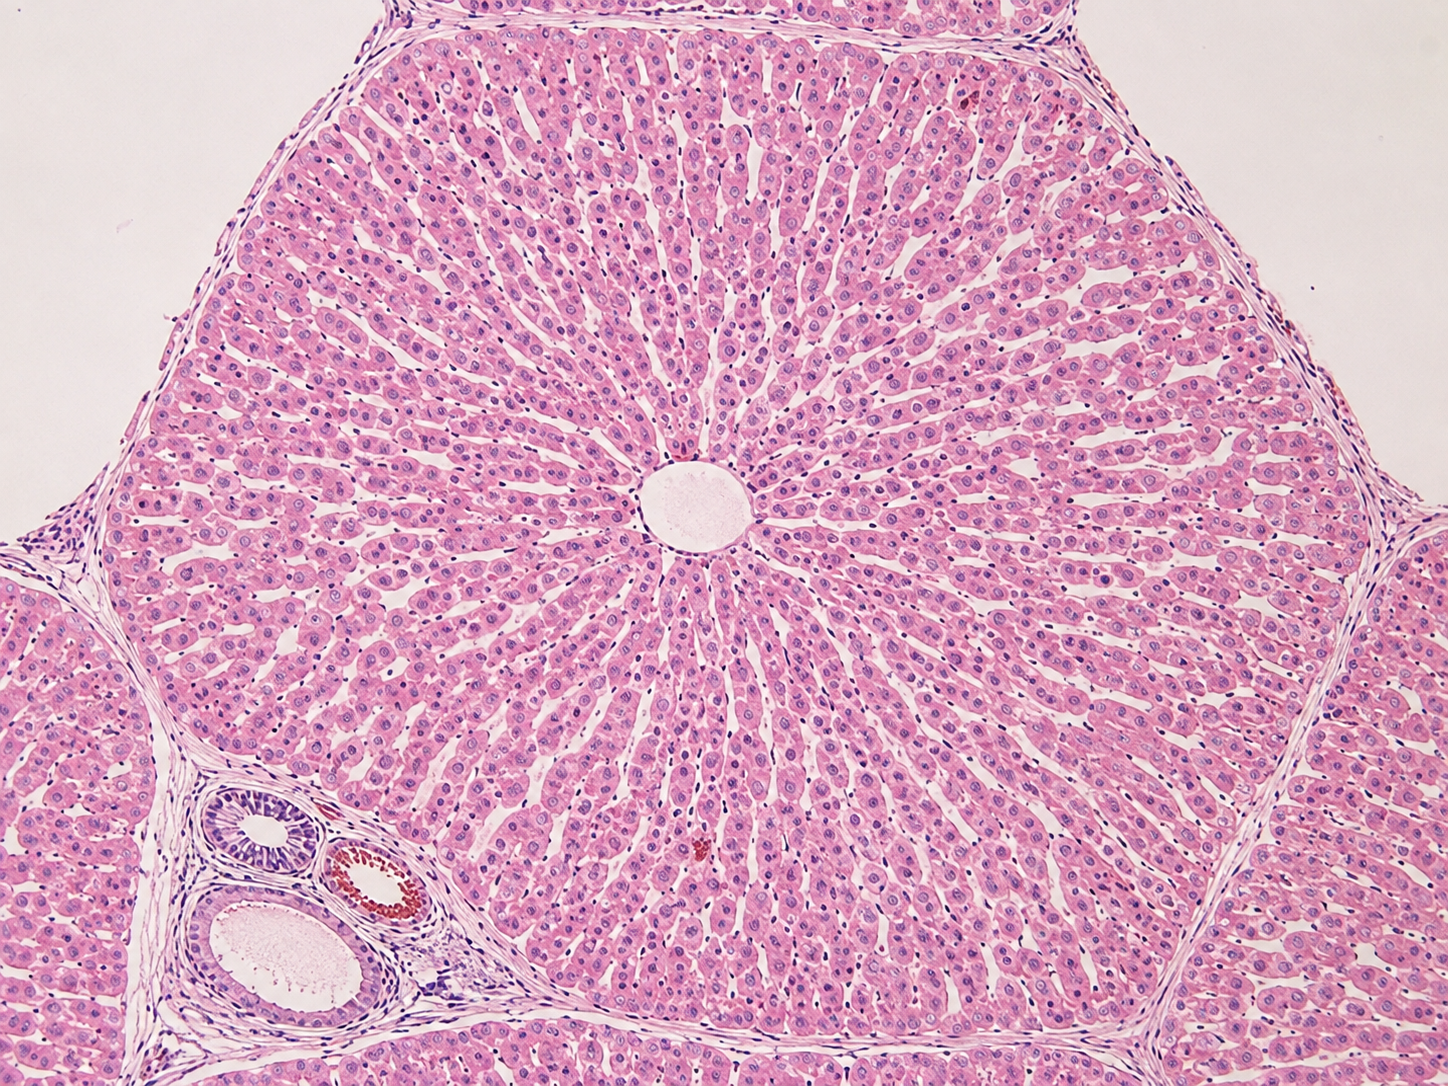
\includegraphics[width=0.52\linewidth]{images/book3/ai/b3-16-liver-lobule-micrograph.png}

{\small Een leverlobje: platen hepatocyten die vanuit een centrale ader uitstralen
en worden omspoeld door bloed uit de darm. Deze \omterm{def:b1:cell-unit-of-life:cell}{cellen} slaan \omterm{def:b1:carbohydrates:polysaccharide}{glycogeen} op, maken
glucose, bouwen \omterm{def:b1:lipids:triglyceride}{vet} en ketonlichamen, en werken stikstof weg --- het metabole
verdeelstation van het lichaam.}
\end{omfigure}

\begin{method}[Een metabole toestand lezen]\label{met:b1:biosyntheses-integration:state}
\begin{enumerate}
  \item Vraag welke brandstof overvloedig is: veel glucose betekent opslag
        (\omterm{def:b1:carbohydrates:polysaccharide}{glycogeen}, daarna \omterm{def:b1:lipids:triglyceride}{vet}); weinig glucose betekent mobilisatie.
  \item Volg de signalen: insuline activeert de synthasen en schakelt het
        fosforylase en het lipase uit; glucagon doet het omgekeerde ---
        meestal via fosforylering van diezelfde \omterm{def:b1:enzymes:enzyme}{enzymen}
        (\cref{ch:b1:enzymes}).
  \item Controleer de kruispunten: \omterm{def:b1:water-small-molecules:atp}{ATP} en citraat blokkeren PFK en openen
        de \omterm{def:b1:biosyntheses-integration:gluconeogenesis}{gluconeogenese}; AMP doet het tegenovergestelde; malonyl-CoA
        blokkeert de vetverbranding terwijl er \omterm{def:b1:lipids:triglyceride}{vet} wordt gemaakt;
        \omterm{def:b1:respiration-fermentation:pdh}{acetyl-CoA} activeert het carboxylase dat de \omterm{def:b1:biosyntheses-integration:gluconeogenesis}{gluconeogenese}
        begint.
  \item Wijs de \omterm{def:b1:mammal-organization:organ}{organen} toe: lever (slaat glucose op, maakt haar en voert
        haar uit; maakt ketonen en ureum), spier (slaat \omterm{def:b1:carbohydrates:polysaccharide}{glycogeen} voor
        zichzelf op, voert lactaat en alanine uit), vetweefsel (slaat \omterm{def:b1:lipids:triglyceride}{vet}
        op en geeft het vrij), hersenen (verbranden glucose, daarna
        ketonen).
\end{enumerate}
\end{method}

\section{De geïntegreerde plant}

\begin{proposition}[Bron en put]\label{prop:b1:biosyntheses-integration:sourcesink}
Overdag voeren de \omterm{def:b1:eukaryotic-cell:plastid}{chloroplasten} van een \omterm{def:b1:flowering-plant-organization:organs}{blad} triosefosfaat uit naar het \omterm{def:b1:eukaryotic-cell:organelle}{cytosol},
waar er \emph{sucrose} van wordt gemaakt voor uitvoer in het floëem
(\cref{ch:b1:plant-transport}) naar de \omterm{def:b1:flowering-plant-organization:organs}{wortels}, de vruchten en de groeiende toppen;
wat het floëem niet kan meenemen blijft in de chloroplast achter als
\emph{\omterm{def:b1:carbohydrates:polysaccharide}{zetmeel}}, een tijdelijke voorraad, die 's nachts wordt gemobiliseerd om de
sucrose te laten doorstromen. Waar de lever van een zoogdier met hormonen tussen
\omterm{def:b1:carbohydrates:polysaccharide}{glycogeen} en uitvoer beslist, beslist een \omterm{def:b1:flowering-plant-organization:organs}{blad} tussen \omterm{def:b1:carbohydrates:polysaccharide}{zetmeel} en sucrose aan de
hand van het fosfaatgehalte in het \omterm{def:b1:eukaryotic-cell:organelle}{cytosol}, dat de uitvoerder van de
chloroplastenvelop aanstuurt. Een plant regelt per \omterm{def:b1:mammal-organization:organ}{orgaan} met de concentraties van
haar eigen metabolieten; het zoogdier legt daar een zenuwlijke en hormonale
aansturing van het geheel bovenop.
\end{proposition}

\begin{omfigure}
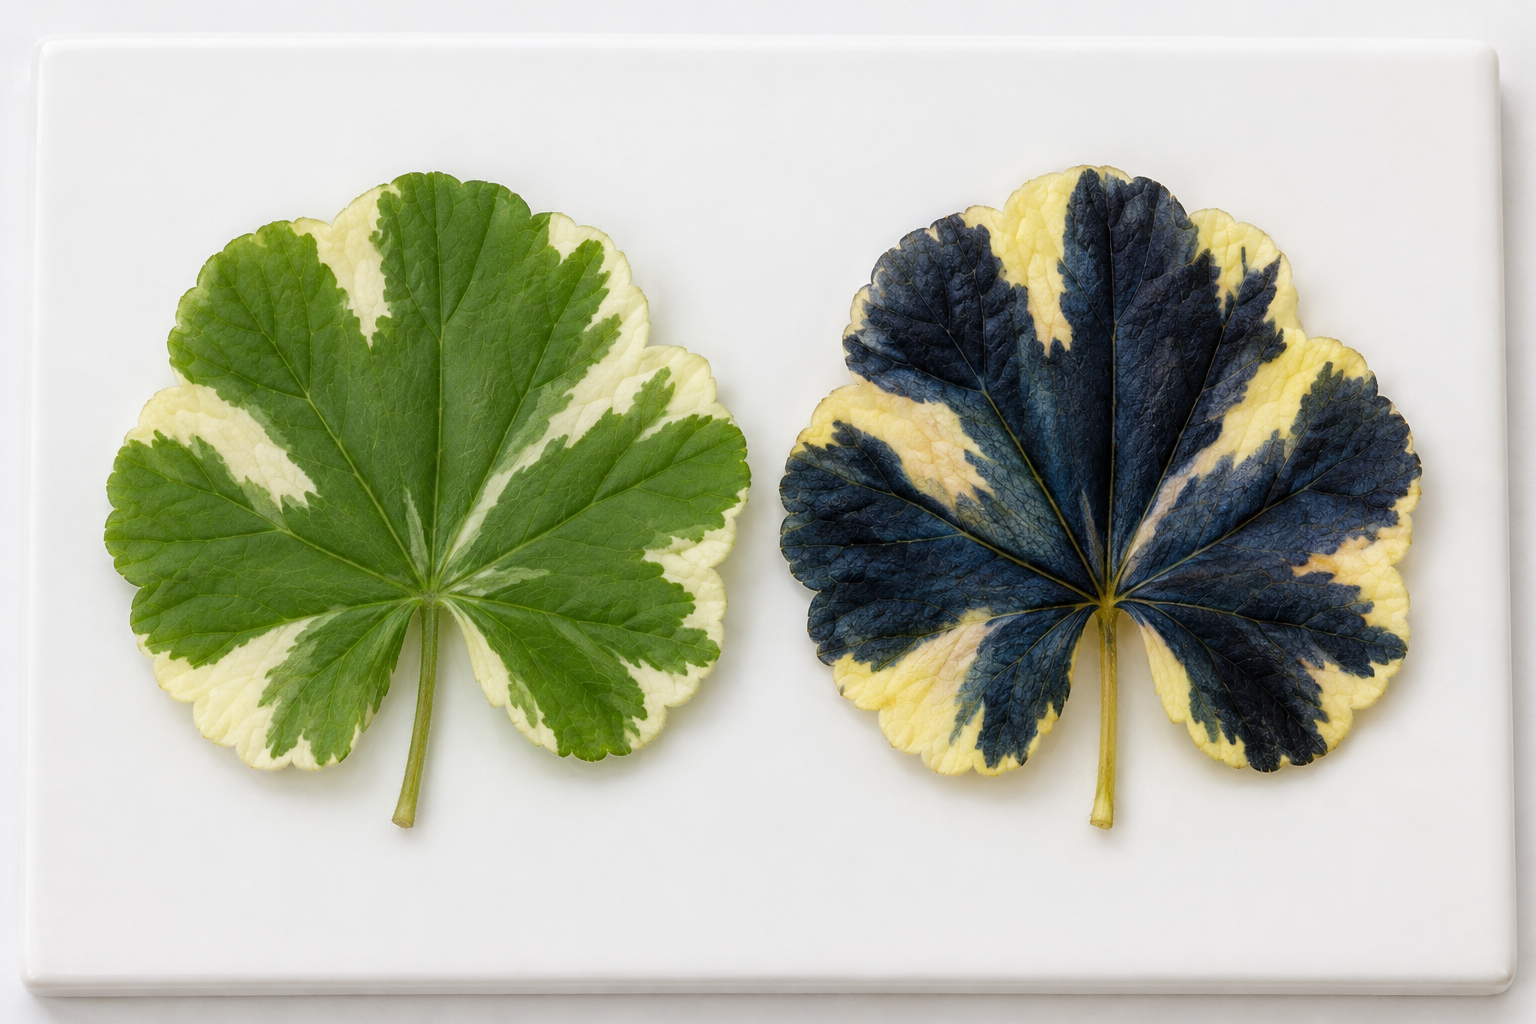
\includegraphics[width=0.6\linewidth]{images/book3/ai/b3-16-variegated-leaf-iodine.png}

{\small Een bont \omterm{def:b1:flowering-plant-organization:organs}{blad} vóór en na de jodiumproef: er is alleen \omterm{def:b1:carbohydrates:polysaccharide}{zetmeel}
(blauwzwart) gemaakt waar \omterm{def:b1:photosynthesis:pigments}{chlorofyl} zat. De witte gebieden, die sucrose uit de
groene invoerden, maakten zelf geen \omterm{def:b1:carbohydrates:polysaccharide}{zetmeel}.}
\end{omfigure}

\begin{example}[Het zetmeel van een nacht]\label{ex:b1:biosyntheses-integration:nightstarch}
Een \omterm{def:b1:flowering-plant-organization:organs}{blad} legt ongeveer de helft van wat het overdag vastlegt als \omterm{def:b1:carbohydrates:polysaccharide}{zetmeel} opzij en
breekt dat de nacht door met een vrijwel constante snelheid af, zodat de voorraad
net vóór zonsopgang op is: verkort men de nacht kunstmatig, dan blijft er \omterm{def:b1:carbohydrates:polysaccharide}{zetmeel}
over; verlengt men hem, dan verhongert de plant in de laatste uren. De snelheid
wordt binnen het eerste uur duisternis afgestemd op de omvang van de voorraad en de
verwachte lengte van de nacht --- een berekening die met \omterm{def:b1:enzymes:enzyme}{enzymen} en een klok wordt
gemaakt, in een \omterm{def:b1:cell-unit-of-life:cell}{cel} zonder brein.
\end{example}

\section{Opgaven}

\begin{exercise}[$\star$]\label{exo:b1:biosyntheses-integration:1}
Noem de drie dingen die een biosynthese nodig heeft en de route die het grootste
deel van het \omterm{def:b1:biosyntheses-integration:ppp}{NADPH} van een dierlijke \omterm{def:b1:cell-unit-of-life:cell}{cel} levert.
\end{exercise}

\begin{exercise}[$\star$]\label{exo:b1:biosyntheses-integration:2}
Noem de drie onomkeerbare stappen van de \omterm{def:b1:respiration-fermentation:glycolysis}{glycolyse} en het \omterm{def:b1:enzymes:enzyme}{enzym} dat elk ervan bij
de \omterm{def:b1:biosyntheses-integration:gluconeogenesis}{gluconeogenese} omzeilt.
\end{exercise}

\begin{exercise}[$\star$]\label{exo:b1:biosyntheses-integration:3}
Lees uit de figuur van de bloedglucose de piek na het ontbijt af, de tijd tot de
terugkeer naar \qty{5}{mmol/L}, en de laagste waarde in de nacht.
\end{exercise}

\begin{exercise}[$\star$]\label{exo:b1:biosyntheses-integration:4}
Waarom kan een kiemende zonnebloemzaadje suiker uit zijn \omterm{def:b1:lipids:triglyceride}{olie} maken en een
hongerend mens niet?
\end{exercise}

\begin{exercise}[$\star\star$]\label{exo:b1:biosyntheses-integration:5}
Bereken de ATP-kosten van het maken van één glucose uit twee lactaat, en de netto
kosten van één ronde van de coricyclus (de spier wint 2, de lever geeft 6 uit). Wie
betaalt, en waarmee?
\end{exercise}

\begin{exercise}[$\star\star$]\label{exo:b1:biosyntheses-integration:6}
Eén palmitaat vraagt 8 \omterm{def:b1:respiration-fermentation:pdh}{acetyl-CoA}, 7 \omterm{def:b1:water-small-molecules:atp}{ATP} en 14 \omterm{def:b1:biosyntheses-integration:ppp}{NADPH}. Hoeveel glucosemoleculen
moeten er door de \omterm{def:b1:respiration-fermentation:glycolysis}{glycolyse} en het pyruvaatdehydrogenase om het \omterm{def:b1:respiration-fermentation:pdh}{acetyl-CoA} te
leveren, en hoeveel door de \omterm{def:b1:biosyntheses-integration:ppp}{pentosefosfaatroute} (2 \omterm{def:b1:biosyntheses-integration:ppp}{NADPH} per stuk) om het \omterm{def:b1:biosyntheses-integration:ppp}{NADPH} te
leveren?
\end{exercise}

\begin{exercise}[$\star\star$]\label{exo:b1:biosyntheses-integration:7}
Leg uit waarom de \omterm{def:b1:biosyntheses-integration:fasynthesis}{vetzuursynthese} en de $\beta$-oxidatie andere \omterm{def:b1:enzymes:enzyme}{enzymen}, andere
compartimenten en andere \omterm{def:b1:enzymes:enzyme}{co-enzymen} gebruiken, en hoe malonyl-CoA verhindert dat
zij samen lopen.
\end{exercise}

\begin{exercise}[$\star\star$]\label{exo:b1:biosyntheses-integration:8}
Schrijf de \omterm{def:b1:biosyntheses-integration:nitrogen}{transaminering} van alanine met $\alpha$-ketoglutaraat op en noem de
producten. Welke richting loopt er na een eiwitmaaltijd, en welke tijdens vasten?
\end{exercise}

\begin{exercise}[$\star\star$]\label{exo:b1:biosyntheses-integration:9}
Een patiënt mist glucose-6-fosfatase. Voorspel met redenen de gevolgen voor de
bloedglucose tussen de maaltijden, voor de grootte van de lever, en voor het
lactaat in het bloed.
\end{exercise}

\begin{exercise}[$\star\star\star$]\label{exo:b1:biosyntheses-integration:10}
De hersenen hebben \qty{120}{g} glucose per dag nodig en \qty{1}{g} \omterm{def:b1:proteins:peptide}{eiwit} levert
\qty{0.55}{g} glucose. Bereken hoeveel \omterm{def:b1:proteins:peptide}{eiwit} een vastende persoon per dag zou
verliezen om de hersenen alleen met \omterm{def:b1:biosyntheses-integration:gluconeogenesis}{gluconeogenese} te voeden, en hoeveel spier dat
voorstelt (\qty{20}{\%} \omterm{def:b1:proteins:peptide}{eiwit}). Leg uit wat ketonlichamen veranderen, als zij de
glucosebehoefte van de hersenen tot \qty{40}{g} terugbrengen.
\end{exercise}

\begin{exercise}[$\star\star\star$]\label{exo:b1:biosyntheses-integration:11}
Insuline activeert het glycogeensynthase en schakelt het glycogeenfosforylase uit;
glucagon doet het omgekeerde. Leg uit waarom beide niet tegelijk actief kunnen
zijn, wat er zou gebeuren als dat wel zo was (bereken het \omterm{def:b1:water-small-molecules:atp}{ATP} dat per cyclus wordt
verspild: één UTP om een glucose toe te voegen, niets om haar te verwijderen), en
waar deze ``zinloze cyclus'' voor wordt gebruikt bij hommels die hun vliegspieren
opwarmen.
\end{exercise}

\begin{exercise}[$\star\star\star$]\label{exo:b1:biosyntheses-integration:12}
``Een \omterm{def:b1:cell-unit-of-life:cell}{cel} heeft geen plan; zij heeft kranen.'' Bespreek dat in een alinea: de
allosterische en hormonale regeling van de kruispuntenzymen, de rol van
afzonderlijke \omterm{def:b1:enzymes:enzyme}{enzymen} voor tegengestelde richtingen, en wat daaruit ontstaat dat op
een plan lijkt.
\end{exercise}

\section{Vraagstuk: vierentwintig uur van een mens}

\begin{problem}[{Weekendvraagstuk --- een dag zonder ontbijt: de voorraden gewogen,
de hersenen gevoed, het eiwit geteld en het vet gemobiliseerd, eindigend op het
aantal uren vasten dat het glycogeen van de lever kan dekken}]
\label{pb:b1:biosyntheses-integration:1}
Een volwassene van \qty{70}{kg} verbruikt per dag \qty{8.4}{MJ} (gemiddeld
\qty{100}{W}) en bezit: leverglycogeen \qty{100}{g}, spierglycogeen \qty{400}{g},
\omterm{def:b1:lipids:triglyceride}{vet} \qty{12}{kg}, \omterm{def:b1:proteins:peptide}{eiwit} \qty{10}{kg} (waarvan \qty{6}{kg} in spier). De hersenen
gebruiken \qty{120}{g} glucose per dag (\qty{5}{g/h}); de overige
glucose-afhankelijke \omterm{def:b1:body-plans-tissues:tissue}{weefsels} (rode \omterm{def:b1:cell-unit-of-life:cell}{cellen}, niermerg) \qty{40}{g}. Energie:
\omterm{def:b1:carbohydrates:monosaccharide}{koolhydraat} \qty{17}{kJ/g}, \omterm{def:b1:lipids:triglyceride}{vet} \qty{38}{kJ/g}, \omterm{def:b1:proteins:peptide}{eiwit} \qty{17}{kJ/g}; \qty{1}{g}
\omterm{def:b1:proteins:peptide}{eiwit} levert via \omterm{def:b1:biosyntheses-integration:gluconeogenesis}{gluconeogenese} \qty{0.55}{g} glucose; \qty{1}{g} \omterm{def:b1:lipids:triglyceride}{vet} levert
\qty{0.1}{g} glucose (uit zijn glycerol).

\medskip
\noindent\textbf{Deel I --- De voorraden.}
\begin{enumerate}
  \item Bereken de energie in elk van de vier voorraden, in megajoule, en
        het aantal dagen verbruik dat elk voorstelt.
  \item Welke voorraad kan rechtstreeks glucose aan het bloed leveren?
        Waarom het spierglycogeen niet?
  \item Bereken de totale glucose die het lichaam per dag voor zijn
        glucose-afhankelijke \omterm{def:b1:body-plans-tissues:tissue}{weefsels} nodig heeft.
  \item Bereken de glucose in het bloed zelf (\qty{5}{mmol/L}, \qty{5}{L},
        \qty{180}{g/mol}) en het aantal minuten dat die de hersenen alleen
        zou voeden.
  \item Welk deel van het dagelijkse verbruik is de glucose van de
        hersenen?
  \item Na een maaltijd is het \omterm{def:b1:carbohydrates:polysaccharide}{glycogeen} van de lever vol en stijgt de
        bloedglucose nog. Noem de volgende bestemming van de glucose en
        het hormoon dat haar daarheen stuurt.
\end{enumerate}

\medskip
\noindent\textbf{Deel II --- De nacht.}
De laatste maaltijd eindigt om 20:00 uur; vanaf dan levert de lever als enige de
glucose van het bloed.
\begin{enumerate}[resume]
  \item Wat is bij \qty{160}{g} glucose per dag de behoefte per uur van de
        glucose-afhankelijke \omterm{def:b1:body-plans-tissues:tissue}{weefsels}?
  \item Hoe lang houdt \qty{100}{g} leverglycogeen het bij die snelheid
        vol, als niets anders glucose levert?
  \item In werkelijkheid levert de \omterm{def:b1:biosyntheses-integration:gluconeogenesis}{gluconeogenese} vanaf de eerste uren
        ongeveer een derde van de glucose. Bereken de duur van het
        \omterm{def:b1:carbohydrates:polysaccharide}{glycogeen} opnieuw.
  \item Op welk tijdstip in de ochtend raakt het leverglycogeen volgens
        elk van beide schattingen op?
  \item De spieren verbranden ondertussen \omterm{def:b1:lipids:fattyacid}{vetzuren}. Bereken het \omterm{def:b1:lipids:triglyceride}{vet} dat
        's nachts (\qty{12}{h}) wordt geoxideerd als zij \qty{60}{\%} van
        het rustverbruik voor hun rekening nemen en alleen \omterm{def:b1:lipids:triglyceride}{vet} verbranden.
\end{enumerate}

\medskip
\noindent\textbf{Deel III --- De volgende dag, zonder eten.}
\begin{enumerate}[resume]
  \item Met het \omterm{def:b1:carbohydrates:polysaccharide}{glycogeen} op moet de \qty{160}{g} glucose uit de
        \omterm{def:b1:biosyntheses-integration:gluconeogenesis}{gluconeogenese} komen. Bereken het \omterm{def:b1:proteins:peptide}{eiwit} dat daarvoor per dag nodig
        is, en de massa spier die dat voorstelt.
  \item Bereken het \omterm{def:b1:water-small-molecules:atp}{ATP} dat de lever uitgeeft om \qty{160}{g} glucose uit
        pyruvaat te maken (6 \omterm{def:b1:water-small-molecules:atp}{ATP} per glucose) en de energie daarvan bij
        \qty{50}{kJ/mol}.
  \item Bereken de bijdrage van de glycerol van het \omterm{def:b1:lipids:triglyceride}{vet}: hoeveel \omterm{def:b1:lipids:triglyceride}{vet} wordt
        er per dag geoxideerd als het al het niet-glucoseverbruik dekt, en
        hoeveel glucose levert de glycerol daarvan?
  \item Bereken het benodigde \omterm{def:b1:proteins:peptide}{eiwit} opnieuw, met de bijdrage van de
        glycerol eraf.
  \item Hoeveel dagen duurt het bij die snelheid tot de helft van de spier
        weg is?
  \item Vanaf de derde dag maakt de lever ketonlichamen en halen de
        hersenen twee derde van hun energie daaruit; de glucosebehoefte
        daalt tot \qty{40}{g} voor de hersenen plus \qty{40}{g} voor de
        rest. Bereken het eiwitverlies per dag en het aantal dagen tot de
        helft van de spier weg is opnieuw.
  \item Bereken hoeveel dagen de vetvoorraad het volhoudt bij \qty{8.4}{MJ}
        per dag (bij langdurig vasten daalt dat tot \qty{6.5}{MJ}: bereken
        dat ook).
  \item Leg uit waarom een vastende persoon aan eiwitverlies sterft voordat
        het \omterm{def:b1:lipids:triglyceride}{vet} op is, en wat ketonlichamen uitstellen.
\end{enumerate}

\medskip
\noindent\textbf{Deel IV --- De kranen.}
\begin{enumerate}[resume]
  \item Noem het \omterm{def:b1:enzymes:enzyme}{enzym} van de lever dat om 03:00 uur actief moet zijn en om
        09:00 uur inactief, en het \omterm{def:b1:enzymes:enzyme}{enzym} dat het omgekeerde moet doen, voor
        het \omterm{def:b1:carbohydrates:polysaccharide}{glycogeen}.
  \item Noem het signaal (hormoon) dat ze elk in hun stand zet, en de
        chemische wijziging waarlangs het werkt.
  \item Een levercel heeft om 03:00 uur veel \omterm{def:b1:respiration-fermentation:pdh}{acetyl-CoA} uit de
        vetoxidatie. Noem het \omterm{def:b1:enzymes:enzyme}{enzym} van de \omterm{def:b1:biosyntheses-integration:gluconeogenesis}{gluconeogenese} dat dit
        activeert en het \omterm{def:b1:enzymes:enzyme}{enzym} van de \omterm{def:b1:respiration-fermentation:glycolysis}{glycolyse} dat \omterm{def:b1:water-small-molecules:atp}{ATP} tegelijk remt.
  \item Leg uit waarom de \omterm{def:b1:biosyntheses-integration:gluconeogenesis}{gluconeogenese} en de \omterm{def:b1:respiration-fermentation:glycolysis}{glycolyse}, tegelijk in
        dezelfde \omterm{def:b1:cell-unit-of-life:cell}{cel} lopend, alleen \omterm{def:b1:water-small-molecules:atp}{ATP} in warmte zouden omzetten, en hoe
        de afzonderlijke \omterm{def:b1:enzymes:enzyme}{enzymen} bij de drie omleidingen dat verhinderen.
  \item Een diabeticus zonder insuline heeft een hoge bloedglucose en toch
        blijft de lever glucose en ketonlichamen maken. Verklaar die
        tegenstrijdigheid uit de kranen.
  \item Geef het resultaat: het aantal uren vasten dat het leverglycogeen
        dekt (met en zonder \omterm{def:b1:biosyntheses-integration:gluconeogenesis}{gluconeogenese}), het dagelijkse eiwitverlies
        vóór en na de overgang naar ketonlichamen, en het aantal dagen dat
        de vetvoorraad het volhoudt.
\end{enumerate}
\end{problem}
